\documentclass{beamer}
\usetheme{Warsaw}
\setbeamercolor{structure}{fg=red!90!black}

\usepackage[utf8]{inputenc}
\usepackage{geometry, amsthm, amsmath, amsfonts, amssymb}
\usepackage{graphicx, paracol, algorithm, listings}
\usepackage[noend]{algpseudocode}

\addtobeamertemplate{footline}{\insertframenumber}

\everymath{\displaystyle}

\title{IA 316: Recommender Systems}
\author{Nicolas Scotto Di Perto and Valentin Charvet}
\institute{Télécom ParisTech}
\date{February 28, 2019}

\begin{document}
\begin{frame}
	\titlepage
\end{frame}

\begin{frame}
	\frametitle{Presentation Of The Environment}
	%The objective of this project is to recommend items to users based on prior knowledge of the database. 
	The objective of this project is to model the behavior of buyers in a simulated retail environment:
	\begin{itemize}\itemsep=2ex
		\item a set of users $\mathcal{U}$
		\item a set of items $\mathcal{I}$
		\item at each time step $t$, a user buys an item among a set $s_t$
		%\item a prediction model 
		%$F(u \in \mathcal{U}, s_t) = i \in \mathcal{I} $
	\end{itemize} 
	We want to learn a function $\hat{f}: (\mathcal{U}, \mathcal{I}^k)  \rightarrow \mathcal{I}$
\end{frame}

\begin{frame}
	\frametitle{Initialization Of The Environment}
	When resetting the environment, we retrieve a history of transactions, each one of them is modeled by
	\begin{itemize}
		\item a user
		\item a list of available items
		\item an action, which corresponds to the recommended item
		\item the reward from this action, it values 
		\begin{itemize}
			\item the price of the item if the user bought the one that was recommended
			\item $0$ else (the recommendation was incorrect)
		\end{itemize}
	\end{itemize}
\end{frame}

\begin{frame}
	\frametitle{Running the environment}
	We make the recommendations iteratively, at each time step $t$:
	\begin{itemize}
		\item we receive a state $s_t$ that corresponds to a user and a set of available items
		\item we recommend the item output by $\hat{f}(s_t)$
		\item we receive a feedback (the reward) that indicates weather the recommendation was correct
		\item \textit{optional} retrain the model on-line using the feedback
	\end{itemize}
\end{frame}

\begin{frame}
	\frametitle{Data Format}
	\begin{itemize}
	\item a state $s_t$ is represented by an array of $k$ substates, each of them contains
	\begin{itemize}
		\item item id
		\item price
		\item 2 item-specific variables
		\item 1 meta data
	\end{itemize}
	\item each of these substates is given for one user and with two user-specific variables
	\end{itemize}
\end{frame}


\begin{frame}
	\frametitle{Implicit Feedback}
	\begin{itemize}
	\item Contrary to the first and second environment, we don't have access to an explicit feedback from the users
	\item However, we know can extract implicit information from the purchases history:
	\begin{itemize}
		\item if the reward from an action is non zero, we can tag the bought article as "positive", since the user liked it enough to buy it
		\item if the reward is 0, we tag the item as "negative" since the user preferred another one despite the recommendation 
	\end{itemize}
	\item Therefore, we can use an inference model using this pseudo explicit feedback
	\item the rate of good recommendations in the history is 
	$29.6 \pm 1.3 \%$
	\end{itemize}
\end{frame}

\begin{frame}
	\frametitle{Cold Start Issue}
	\begin{itemize}
		\item During the runs, we frequently encounter users that did not appear in the history dataset (usually a dozen)
		\item Therefore, we need to use the users metadata to be able to make predictions for those new users
		\begin{itemize}
			\item For a new user $u_{new}$, we look for the most similar to him in $\mathcal{U}$ using cosine similarity with users variables
			\item \textit{First Method:} we recommend the same item we would have done to the most similar user
			\item \textit{Second Method:} we use the embedding of the most similar user to make the prediction for the new one
		\end{itemize}
	\end{itemize}
\end{frame}

\begin{frame}
	\frametitle{User Based Recommendation}
	\begin{itemize}
	\item For this model, we only retrieve the positive recommendations from the history
	\item at each time step, we receive $u\in \mathcal{U}$ and $i_1 \dots i_k \in \mathcal{I}^k$
	\item we compute the cosine similarity between $u$ and the users in the history that have bought an item from $i_1 \dots i_k$
	\item we recommend the most expensive item from those having the highest similarities
	\item It enables solving the cold start problem easily
	\end{itemize}
\end{frame}

\begin{frame}
	\frametitle{Implicit Feedback + User Based}
	\begin{itemize}
	\item As said previously, the implicit feedback model fails at recommending items for new users as it embeds unseen values
	\item at time step $t$ if we encounter a unseen user, we look for the most similar one
	\item we use the embedding from the similar (already seen) user as input of the neural network
	\end{itemize}
\end{frame}

\begin{frame}
	\frametitle{Evaluation Metrics}
	To assess the performance of our model, we need to define a metric
	\begin{itemize}
		\item A naive way to do this is to measure the rate of correct predictions ie count the number of positive rewards during a run
		\item However, from a business point of view, we want to maximize the mean reward $\bar{R}$. If 
		$\bar{R} > \frac{1}{30}\times \underset{i \in \mathcal{I}}{max}\lbrace price(i)\rbrace$(reward if we always recommend the most expensive item) then our model performed well 
	\end{itemize}
\end{frame}

\begin{frame}
	\frametitle{Experimental Results}
	\begin{figure}
	\centering
	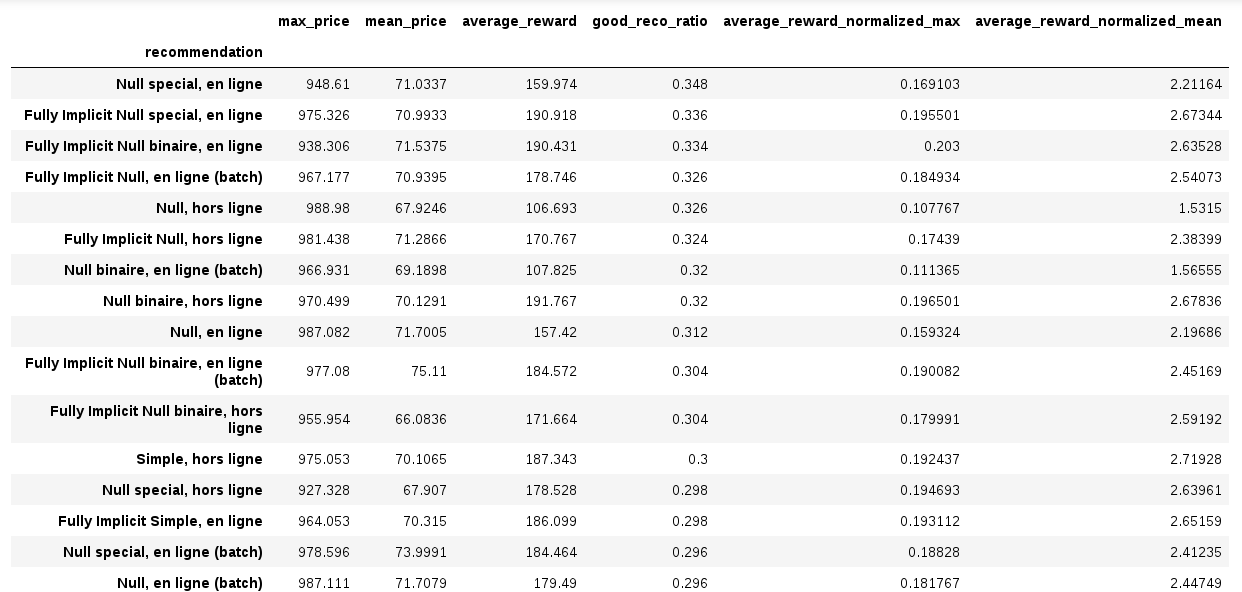
\includegraphics[width=\textwidth]{resultats.png}
	\caption{Results with our different metrics for several models}	
	\end{figure}

	
	%\begin{tabular}{c ||c|c}
	%	Model & Mean Reward & $\tau_{correct}$ \\
	%	\hline
	%	Raw Implicit Feedback & 71.1 & 23.5\% \\
	%	User Based & 147 & 28.9\% \\
	%	Implicit Feedback + User Similarity & 0 & 0 \\
	%\end{tabular}
\end{frame}


\end{document}